\chapter{系统构建与测试验证}\label{chap:build-validation}

系统移植是否完成，需要通过可重复的构建流程和可观察的运行结果确认。当前系统需要编译 Rust 内核，交叉编译 C 用户库、Shell 和用户程序，生成包含内核、用户程序和文件系统内容的磁盘镜像，并通过 QEMU RISC-V virt 机器启动到可交互 Shell。本章说明当前系统的构建与运行环境、功能测试范围和结果分析，并结合 \verb|main| 分支分析重构后验证对象的变化。

\section{构建与运行环境}

当前仓库采用 Makefile 组织整体构建，用 Cargo 构建 Rust 内核，用 RISC-V 交叉 GCC 构建用户态 C 程序。内核部分在 \verb|src/Makefile| 中调用 \verb|cargo +nightly-2026-04-07 rustc|，目标三元组为 \verb|riscv64gc-unknown-none-elf|，并使用 \verb|-Z build-std=core,alloc,compiler_builtins| 构建裸机所需的标准库子集。Cargo 输出静态库后，Makefile 再用 \verb|rust-lld| 和 \verb|src/kernel-riscv64.ld| 链接生成 \verb|src/kernel.elf|。这种流程与普通用户态 Rust 程序不同，原因在于内核运行在无标准库、无操作系统服务的环境中，只能使用 \verb|core|、\verb|alloc| 和明确接入的底层库。

用户态部分仍由 C 语言实现。用户库 \verb|lib/libv6pptongji.a|、Shell 的 \verb|Shell.exe| 以及 \verb|programs| 目录下的 \verb|ls|、\verb|cat|、\verb|echo|、\verb|cp|、\verb|rm|、\verb|mkdir|、\verb|fork|、\verb|sig| 等程序都通过 \verb|riscv64-unknown-elf-gcc| 编译，并使用 \verb|-march=rv64gc|、\verb|-mabi=lp64d|、\verb|-ffreestanding|、\verb|-nostdlib| 等选项生成独立的 RISC-V ELF64 可执行文件。链接时指定 \verb|-Ttext-segment=0x400000| 和入口 \verb|_start|，与第 5 章中的 ELF 加载地址和用户态 C 运行时入口相对应。

\begin{figure}[htbp]
  \centering
  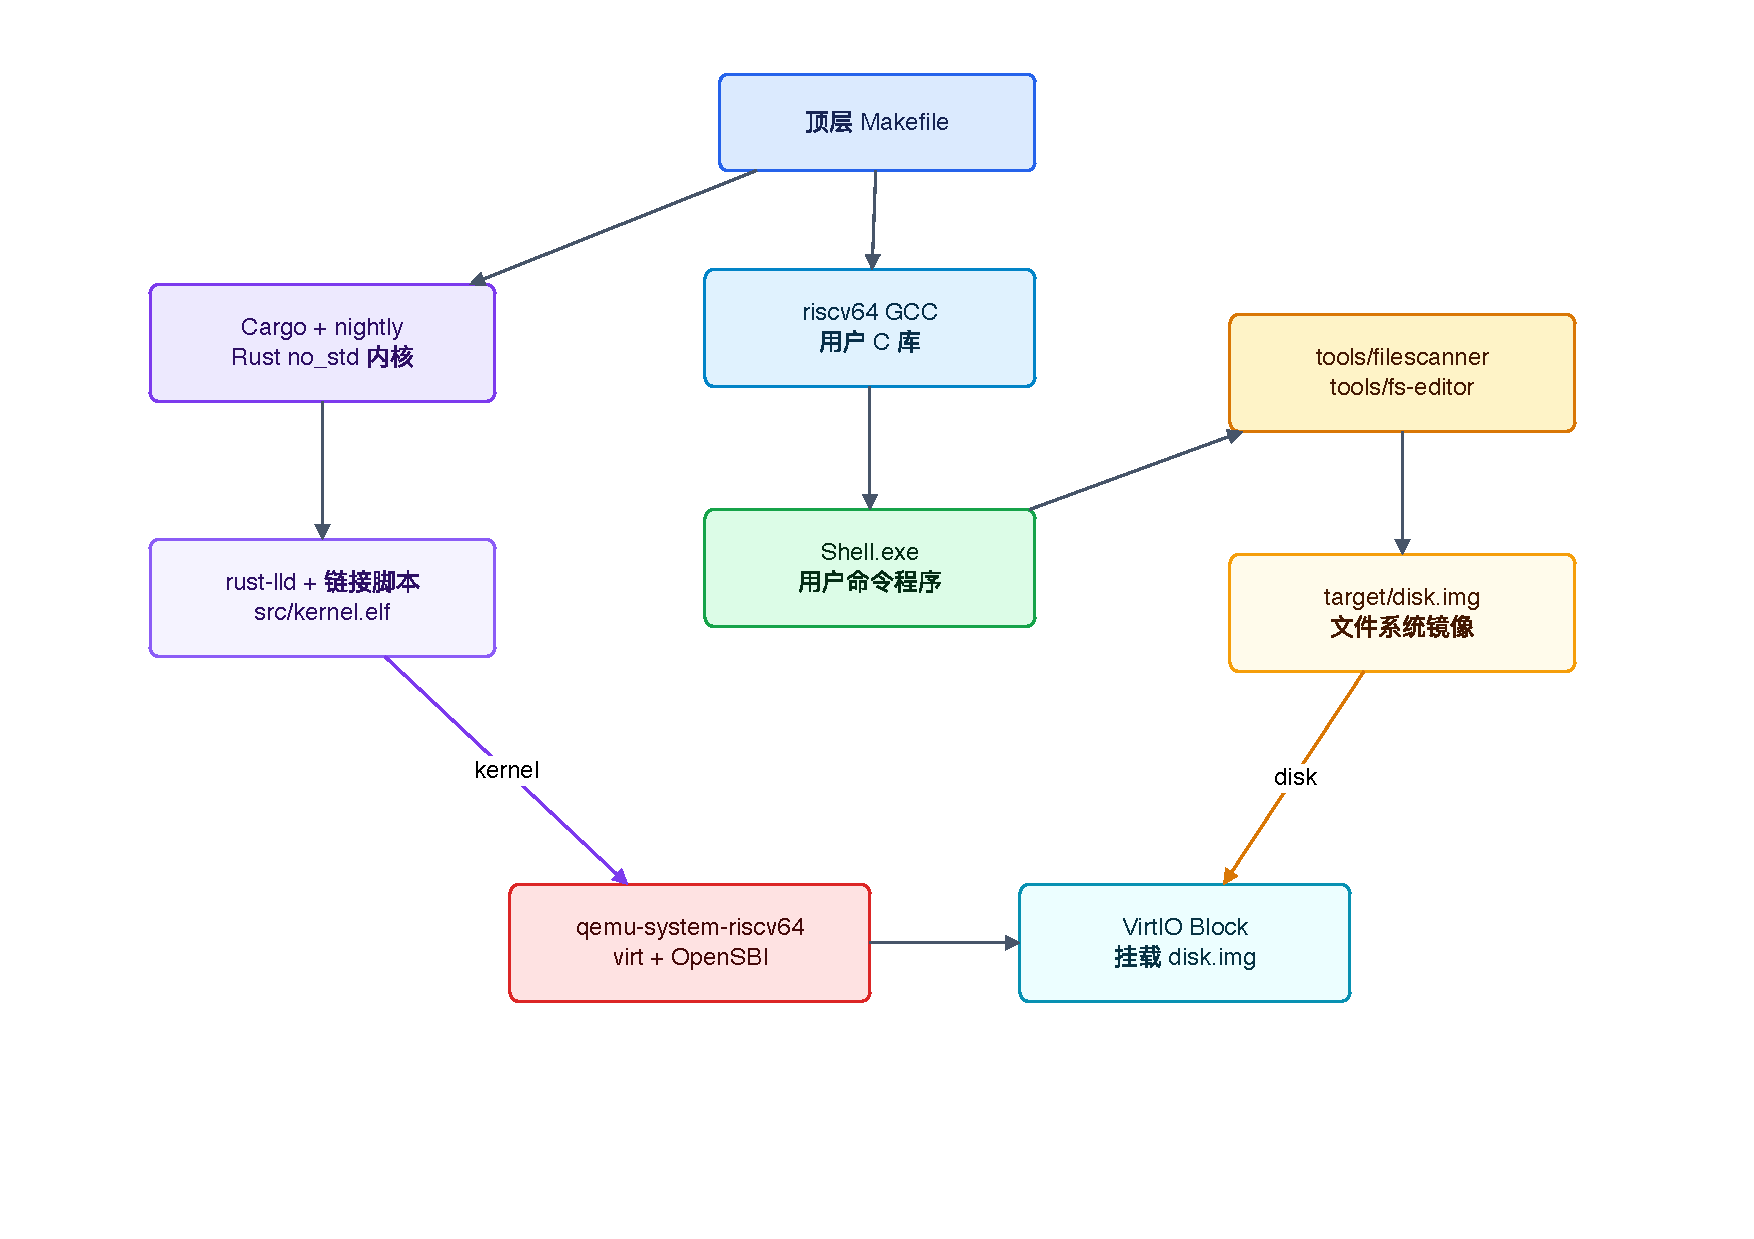
\includegraphics[width=0.95\textwidth]{figures/build-pipeline.pdf}
  \caption{内核、用户程序与磁盘镜像构建流程}\label{fig:build-pipeline}
\end{figure}

\figref{fig:build-pipeline} 展示了当前构建流程。顶层 \verb|make all| 依次构建工具、用户库、Shell、用户程序和内核，并将构建产物复制到 \verb|target/img-workspace|。随后，\verb|tools/filescanner| 扫描工作目录内容，\verb|tools/fs-editor| 生成 \verb|target/disk.img|。运行 RISC-V 目标时，\verb|make qemu-riscv64| 使用 \verb|qemu-system-riscv64|、\verb|-machine virt|、\verb|-bios default|、\verb|-nographic| 和 \verb|-kernel src/kernel.elf| 启动内核，同时通过 VirtIO MMIO 设备挂载 \verb|target/disk.img| 作为块设备后端\cite{qemu_riscv_doc}。

相较 \verb|main| 分支，构建和运行对象发生了三类变化。原版本主要通过 CMake/Ninja 构建 C++ 内核，并通过 \verb|qemu-system-i386| 和 IDE 磁盘启动；当前版本增加 Rust 内核构建链和 RISC-V 运行目标。原用户态程序主要面向 IA-32/PE 或 32 位环境，当前用户态程序统一交叉编译为 ELF64/RISC-V。原系统运行依赖 PC 机器模型中的 BIOS、ATA 和传统中断设备；当前 RISC-V 目标通过 OpenSBI、QEMU virt、PLIC、UART 和 VirtIO Block 完成启动与设备访问。顶层 Makefile 仍保留 \verb|qemu|、\verb|qemug| 等旧目标，便于对比重构前后的平台差异；实际验证当前系统时，重点使用 \verb|qemu-riscv64| 和 \verb|qemu-riscv64g|。

\begin{table}[htbp]
  \centering
  \caption{主要构建与运行目标}\label{tab:build-targets}
  \begin{tabular}{p{0.25\textwidth}p{0.62\textwidth}}
    \toprule
    目标或产物 & 作用 \\
    \midrule
    \verb|src/kernel.elf| & RISC-V/Rust 内核 ELF 文件，由 Cargo 静态库和链接脚本生成 \\
    \verb|target/disk.img| & 包含 Shell、用户程序、设备节点和文件系统内容的磁盘镜像 \\
    \verb|make qemu-riscv64| & 通过 QEMU virt 机器启动当前 RISC-V 系统 \\
    \verb|make qemu-riscv64g| & 以 GDB stub 方式启动，便于远程调试内核 \\
    \verb|make check| & 对 Rust 内核执行交叉目标下的类型检查 \\
    \verb|make qemu| & 保留的 IA-32/QEMU 运行目标，用于对照原平台路径 \\
    \bottomrule
  \end{tabular}
\end{table}

\section{功能测试}

当前系统的验证以 QEMU 中的交互测试为主，辅以构建目标和启动日志检查。启动阶段观察内核是否能通过 OpenSBI 进入 Rust 入口，完成 BSS 清零、页表初始化、串口初始化、物理内存管理初始化、0 号进程创建、Trap 初始化、Buffer 初始化、PLIC 与定时器初始化、文件系统超级块读取、根目录设置和控制台打开。上述步骤通过后，内核会创建 init 进程并执行 \verb|/Shell.exe|，随后在串口终端中显示 Shell 提示符。这一过程验证了第 3 章到第 6 章中多个模块的衔接。

Shell 功能测试围绕常见用户程序展开。\verb|ls| 用于检查目录读取和用户程序执行，\verb|cat|、\verb|echo|、\verb|cp|、\verb|rm|、\verb|mkdir| 用于检查基本文件读写和目录操作，\verb|cd| 及提示符路径变化用于检查当前目录维护。这里把这些命令作为用户态程序经由系统调用访问文件系统的验证样例。命令若能从 \verb|/bin| 查找、由 Shell \verb|fork| 后 \verb|exec|，并正常返回 Shell，便可说明 ELF 加载、文件描述符、进程等待和终端输出路径已经配合工作。

进程管理测试主要关注 \verb|fork|、\verb|exec|、\verb|wait|、\verb|sleep| 和调度返回。仓库中的 \verb|fork.c|、\verb|forks.c|、\verb|performance.c|、\verb|test.c| 等用户程序可以用于观察父子进程返回值、多个子进程并发运行、父进程等待子进程退出以及时间片调度效果。Shell 执行普通命令时也会经过典型进程路径，包括父进程等待、子进程重定向描述符并执行目标程序、程序退出后父进程重新获得提示符。

管道与重定向测试可通过 Shell 的命令树执行路径观察。管道命令调用 \verb|pipe| 创建描述符对，左侧命令复制写端到标准输出，右侧命令复制读端到标准输入；重定向则通过 \verb|open|、\verb|creat|、\verb|close| 和 \verb|dup| 修改标准输入输出。典型样例包括把 \verb|echo| 输出写入文件，再用 \verb|cat| 读取，或用管道连接两个简单命令。该类测试覆盖系统调用层、打开文件表、管道文件对象、Shell 描述符管理和进程生命周期。

信号测试主要包括两类。一类来自用户程序，例如 \verb|sig.c|、\verb|newsig.c|、\verb|sigTest.c| 可安装处理函数、发送信号或进入睡眠等待信号；另一类来自终端控制字符，例如在 Shell 或测试程序运行时输入 Ctrl-C，TTY 层应向相关进程发送 \verb|SIGINT|。用户安装处理函数时，内核应构造信号处理上下文并在 \verb|sigret| 后恢复；用户未安装处理函数时，进程按默认动作结束。该类测试验证第 4 章和第 5 章中异常、系统调用、信号和进程切换的组合路径。

\begin{figure}[htbp]
  \centering
  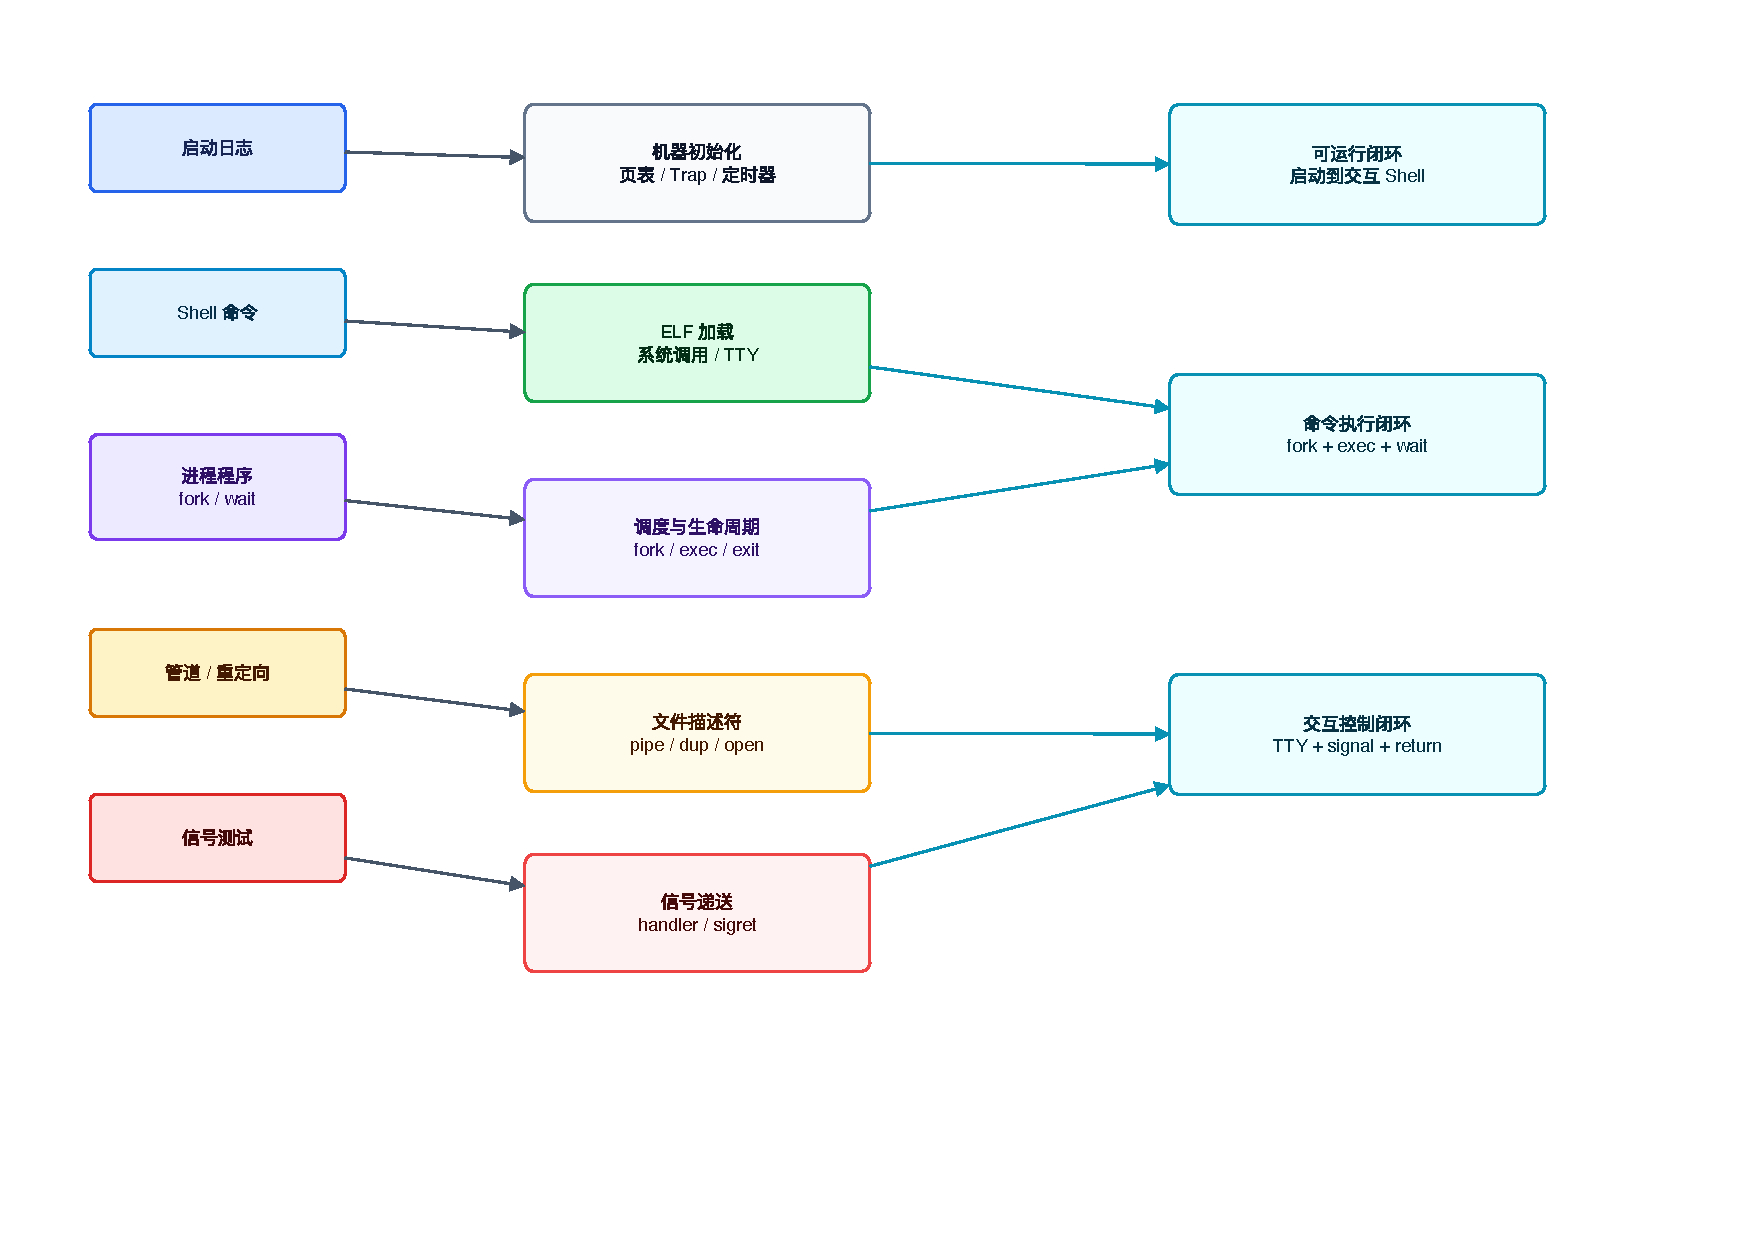
\includegraphics[width=0.95\textwidth]{figures/validation-matrix.pdf}
  \caption{系统功能验证覆盖关系}\label{fig:validation-matrix}
\end{figure}

\figref{fig:validation-matrix} 将测试对象和内核模块对应起来。启动测试覆盖机器初始化、内存管理、Trap 和文件系统挂载；Shell 命令覆盖用户程序加载、系统调用和 TTY；进程类程序覆盖调度与父子进程；管道和重定向覆盖文件描述符与进程协作；信号测试覆盖 TTY、异常和用户态上下文恢复。这些测试尚不能替代完整自动化测试体系，但对于教学操作系统移植而言，可以确认系统已经具备从启动到交互、从命令执行到进程回收的基本运行路径。

\section{结果分析}

从构建结果看，当前系统已经形成面向 RISC-V 的构建链。Rust 内核可以以 \verb|no_std| 方式生成 RISC-V ELF，用户库、Shell 和用户程序可以交叉编译为 ELF64/RISC-V，可执行文件和资源可以写入 Unix V6++ 文件系统镜像，QEMU virt 机器可以通过 OpenSBI 加载内核并挂载 VirtIO 磁盘。上述结果表明，重构工作覆盖了内核语言迁移、用户态程序、镜像制作和仿真运行等工程环节。

功能结果显示，当前系统相较 \verb|main| 分支完成了三类迁移。体系结构由 IA-32/PC 迁移到 RISC-V/QEMU virt，启动、中断、系统调用、页表和设备访问路径均发生变化。内核主体由 C++ 改写为 Rust，进程、文件对象、文本段引用、中断保护等资源的生命周期表达更明确，错误返回也更多通过 \verb|Result| 和枚举呈现。用户态环境保持 Unix V6++ 的 Shell 和常用命令语义，原教学系统的使用方式得以延续。

当前验证仍以手工交互和模块级观察为主，自动化程度有限。文件系统和 Buffer 管理虽然可以支撑基本命令与镜像访问，但其内部一致性、异常恢复和压力场景仍需要更系统的测试；进程退出状态、子进程时间累计等细节仍有简化；部分系统调用保留为空实现或返回 \verb|ENOSYS|。这些限制不影响本文所述的 RISC-V/Rust 移植主线，也说明系统仍处于教学内核的可运行框架阶段，后续需要继续补充自动化测试、压力测试和更完整的 POSIX 语义。
